\section{Durchführung}
\label{sec:Durchführung}


\subsection{Versuchsaufbau}

Der Versuch ist entsprechend \autoref{fig:aufbau} aufgebaut.
Über die Photodiode werden die wandernden Intensitätsmaxima des Interferometers gezählt.
Dabei stellt ein Synchromotor sicher, dass der verschiebbare Spiegel mit einer konstanten Geschwindigkeit so bewegt wird, dass es der Photodiode möglich ist, alle Maxima zu zählen.

\begin{figure}[H]
    \centering
    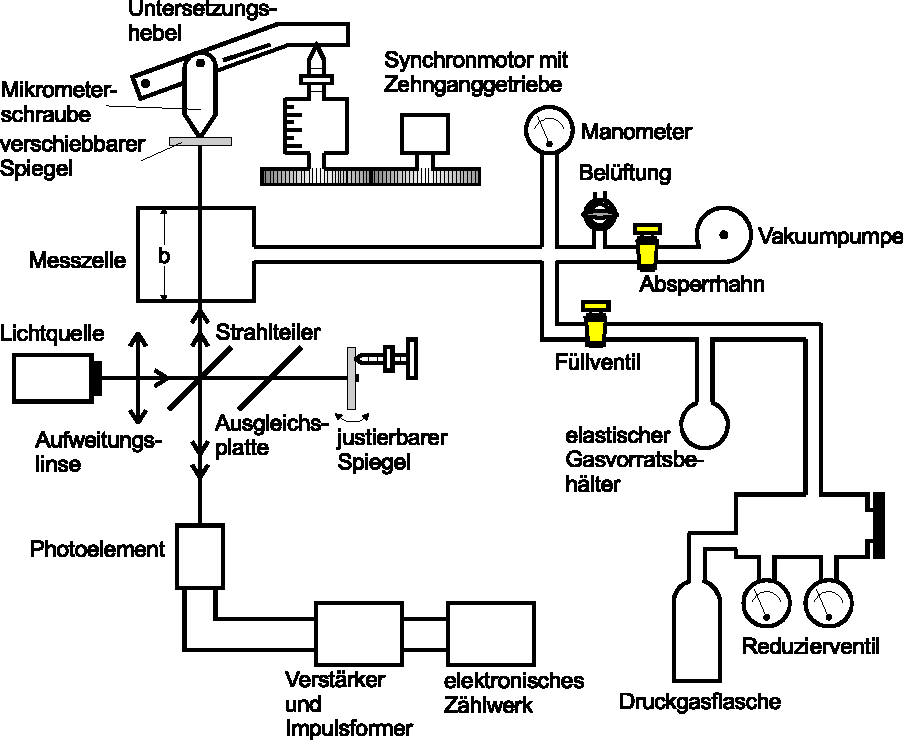
\includegraphics[width = .75\textwidth]{figures/Aufbau.pdf}
    \caption{Schematischer Aufbau der Messapparatur \cite{ap11}.}
    \label{fig:aufbau}
\end{figure}


\subsection{Versuchsdurchführung}

Die Durchführung besteht im Wesentlichen aus zwei Teilen.
Zuerst soll über eine Verschiebung des Spiegels die Wellenlänge des Lasers bestimmt werden. \\

Um zuverlässige Messergebnisse zu erhalten, muss der Aufbau jedoch zu Beginn über die Stellschrauben am nicht verschiebbaren Spiegel so einjustiert werden, 
dass auf einem Blatt Papier vor der Photodiode ungefähr ein Intensitätsminimum und zwei Maxima zu erkennen sind.\\

Zur Messung wird der Spiegel aus einem Abstand von $5 \,\si{\milli\meter}$ auf $10 \,\si{\milli\meter}$ bewegt, wobei zu beachten ist, 
dass diese Entfernungen den Markierungen auf der sich drehenden Schraube entsprechen, nicht der tatsächlichen Distanz, die der Spiegel bewegt wird. \\

Während dieser Bewegung werden an der Photodiode die durchlaufenden Intensitätsmaxima gezählt, die Messung wird weitere neun Mal durchgeführt. \\

Außerdem soll der Brechungsindex von Luft experimentell ermittelt werden.
Dazu wird der Spiegel auf einen konstanten Abstand gebracht.
Der Druck in der Messzelle wird auf knapp $500 \, \si{\milli\meter}\text{Hg}$ gepumpt, der Druck wird auf Atmosphärendruck abgelassen und die Maxima werden erneut gezählt.
Dann wird der Druck, möglichst gleichmäßig und langsam, erneut auf $500 \, \si{\milli\meter}\text{Hg}$ aufgepumpt und die Maxima werden gezählt.
Dieser Vorgang von aufpumpen und Luft ablassen wird solange wiederholt, bis sechs oder sieben Messwerte vorliegen.




